\section{Hitting times at the basepoints}\label{ch:bphit}

The third question, whether $T_1$ is a hitting time, is probabilistic.

We keep the notation of Section~\ref{ch:basepoint}: $\varphi_\alpha(u)=\xi(\alpha)/\xi(\alpha+\sqrt u)$ is the Laplace transform of $T_\alpha$ whenever that variable exists, $b_\alpha=\frac{\xi'}{\xi}(\alpha)$, $v_\alpha(\theta)=\re(\xi'/\xi)(\alpha+i\theta)$, and $\rho_{1/2}=v_1/\pi$ is the Thorin density of $T_1$ in the chart $\theta=\sqrt z$. In addition $B$ is a standard Brownian motion, $H^{(c)}_a$ is the first passage time of $B_t+ct$ to the level $a\ge0$, and $H_a=H^{(0)}_a$; this $H$ has nothing to do with the de Bruijn Newman flow $H_t$ of Section~\ref{ch:dbn}.

\subsection{Kent's theorem and Brownian first passage to a random level}\label{bp:sec:kent}

The first candidate is the hitting time of a level by a diffusion. By Kent's theorem \cite{Kent80} and Krein's inverse spectral theory \cite{DymMcKean76}, recalled in Section~\ref{sec:ch18:kent}, the first hitting times of levels by diffusions started at a reflecting or entrance end are exactly the GGCs without drift whose Thorin measures consist of unit atoms at distinct points, the Dirichlet eigenvalues of the interval up to the level. The Thorin measure of $\varphi_1$ is absolutely continuous, so $T_1$ is not such a hitting time. It is the clock at the centre that has the discrete form: under RH its Thorin measure has an atom at each $\gamma^2$, of mass the multiplicity of the zero, so that it is such a hitting time exactly when the zeros are also simple. Brownian motion offers a second candidate, a first passage to a random level, and Proposition~\ref{prop:nogo} excludes it for the clock.

\begin{proposition}\label{bp:prop:nogo}
For no drift $c\ge0$ and no random level $L\ge0$ independent of the Brownian motion is $T_1$ equal in law to the first passage time $H^{(c)}_L$. (For $c<0$ the first passage time is infinite with positive probability, so equality is impossible.)
\end{proposition}

\begin{proof}
Conditionally on $L$, the Laplace transform of $H^{(c)}_L$ is $\exp\{-L(\sqrt{c^2+2u}-c)\}$, so $\E e^{-uH^{(c)}_L}=\E\exp\{-L(\sqrt{c^2+2u}-c)\}$ extends analytically, and bounded by one, to the region $R_c=\{u:\re\sqrt{c^2+2u}>c\}$, which contains the right half plane and lies inside $\cut$. The function $\varphi_1$ is analytic there as well, by the proof of Proposition~\ref{bp:prop:thorin}, so if the two agreed on $\re u>0$ they would agree on $R_c$, and $|\varphi_1|\le1$ on $R_c$ and on its boundary, the parabola $u_q=\frac12(-q^2+2icq)$, $q\in\R$, on which $\sqrt{c^2+2u_q}=c+iq$, as in the proof of Proposition~\ref{prop:nogo}. On that parabola $\re\sqrt{u_q}$ stays bounded while $\im\sqrt{u_q}\sim q/\sqrt2$, so by Stirling's formula $|\xi(1+\sqrt{u_q})|$ decays exponentially and $|\varphi_1(u_q)|\to\infty$. For $c=0$ the parabola is the cut itself and $|\varphi_1(-t^2)|=|\xi(1)/\xi(1+it)|$, which equals $13.0$, $1.2\times10^4$, $2.0\times10^{10}$ and $1.5\times10^{23}$ at $t=10,20,40,80$, as computed by \texttt{compute.py}.
\end{proof}

A subordinator with a drift as well as a stable one half part escapes this obstruction: on the cut, where $\sqrt u=it$, its exponent $u+\sqrt u=-t^2+it$ has negative real part, so mixtures of its transforms can grow.

\subsection{Subordination of the centre clock}\label{bp:sec:sub}

Let $T$ be the clock variable of Section~\ref{ch:clock}, with $\E e^{-uT}=\varphi_{1/2}(u)=1/G(u)$, a positive random variable that exists with no hypothesis (Theorem~\ref{thm:ch12:idsd}, whose proof uses the verification of RH below height $1000$); it is the clock of \cite{P17}, and we call it the centre clock.

\begin{theorem}\label{bp:thm:sub}
Let $\widetilde T$ have the tilted law $P(\widetilde T\in dt)=e^{-t/4}P(T\in dt)/\E e^{-T/4}$, and let $(\sigma_\ell)_{\ell\ge0}$ be an independent subordinator with Laplace exponent $u+\sqrt u$. Then
\[
T_1\stackrel{d}{=}\sigma_{\widetilde T}\stackrel{d}{=}\widetilde T+H_{\widetilde T/\sqrt2},
\]
where $H_a$ is the first passage time of a standard Brownian motion to the level $a$, independent of $\widetilde T$.
\end{theorem}

\begin{proof}
For $\re\sqrt u\ge0$ the number $\frac12+\sqrt u$ has positive real part and $(\frac12+\sqrt u)^2=\frac14+u+\sqrt u$, so $\xi(1+\sqrt u)=\xi\big(\frac12+\sqrt{\tfrac14+u+\sqrt u}\big)$ with the principal root. Hence
\[
\begin{aligned}
\varphi_1(u)&=\frac{\xi(1)}{\xi(1+\sqrt u)}=\frac{\varphi_{1/2}(\frac14+u+\sqrt u)}{\varphi_{1/2}(\frac14)}\\
&=\frac{\E\big[e^{-T/4}e^{-(u+\sqrt u)T}\big]}{\E e^{-T/4}}=\E e^{-(u+\sqrt u)\widetilde T}=\E e^{-u\sigma_{\widetilde T}} .
\end{aligned}
\]
Finally $\sigma_\ell\stackrel{d}{=}\ell+H_{\ell/\sqrt2}$, because $\E e^{-uH_a}=e^{-a\sqrt{2u}}$.
\end{proof}

The subordinator $\sigma$ has a classical description: a subordinator with exponent $\kappa_1u+\kappa_2\sqrt{2u}$ is the inverse local time at zero of a Brownian motion that is sticky at zero, the drift $\kappa_1$ measuring the time spent at zero per unit of local time \cite[Section 5.7, p.~187]{ItoMcKean65}; here $\kappa_1=1$ and $\kappa_2=1/\sqrt2$. So $T_1$ is the first time the local time at zero of a sticky Brownian motion exceeds an independent level distributed as $\widetilde T$.

\begin{corollary}\label{bp:cor:kent}
Assume RH and that the zeros are simple. Then $\widetilde T$ is Kent's hitting time for a Krein string whose Dirichlet spectrum is $\{\gamma^2+\frac14\}=\{|\rho|^2\}$, and $T_1$ is the first hitting time of the level $y_*$ by the process $D(\ell_t)$, where $D$ is that string diffusion started at its left end, $y_*$ is the level whose hitting time by $D$ is $\widetilde T$, and $\ell_t$ is the local time at zero of an independent sticky Brownian motion $B$. Equivalently, $T_1$ is the first hitting time of the line $\{y=y_*\}$ by the two dimensional Markov process $(D(\ell_t),B_t)$.
\end{corollary}

\begin{proof}
Under RH, $\E e^{-u\widetilde T}=\varphi_{1/2}(\frac14+u)/\varphi_{1/2}(\frac14)=\prod_{\gamma>0}(\gamma^2+\frac14)/(\gamma^2+\frac14+u)$, the product running over the ordinates $\gamma>0$ repeated according to multiplicity. Since the zeros are simple, this is a GGC without drift with unit atoms at the distinct points $|\rho|^2$, so Kent's theorem and Krein's inverse theory provide the string. The first time $D(\ell_t)$ reaches $y_*$ is the first $t$ with $\ell_t\ge\widetilde T$, which is $\sigma_{\widetilde T}$.
\end{proof}

The tail \eqref{bp:eq:tail} follows from the theorem: $P(H_a>x)\sim a\sqrt{2/(\pi x)}$, so $P(T_1>x)\sim\E[\widetilde T]/\sqrt{\pi x}$, and $\E\widetilde T=-\frac{d}{du}\log\varphi_{1/2}(\frac14+u)\big|_{u=0}=\frac{\xi'}{\xi}(1)=\sum_\rho\rho^{-1}$.

\subsection{The density of \texorpdfstring{$T_1$}{T1} and harmonic measure}\label{bp:sec:density}

Conditioning on $\widetilde T$ in Theorem~\ref{bp:thm:sub} and using the density of $H_a$ gives the density of $T_1$ as an expectation over the tilted centre clock,
\begin{equation}\label{bp:eq:density}
f_{T_1}(x)=\E\Big[\frac{\widetilde T}{2\sqrt\pi}\,(x-\widetilde T)^{-3/2}\exp\Big(-\frac{\widetilde T^2}{4(x-\widetilde T)}\Big)\,\mathbf 1\{\widetilde T<x\}\Big],
\end{equation}
since $H_a$ has density $a(2\pi h^3)^{-1/2}e^{-a^2/2h}$ and $a=\widetilde T/\sqrt2$. Figure~\ref{bp:fig:density2} compares \eqref{bp:eq:density}, averaged over $4\times10^5$ draws of $\widetilde T$, against numerical inversion of $\varphi_1$ by Talbot's method \cite{Talbot79} and shows the whole density. At the points computed the two agree to about $0.1\%$, except near the mode, at $x=0.024$, where the Monte Carlo average is within $1\%$. For large $x$ the density behaves like $\frac{1}{2\sqrt\pi}\sum_\rho\rho^{-1}\,x^{-3/2}=0.00652\,x^{-3/2}$, the derivative of \eqref{bp:eq:tail}. Near the origin the density is super flat, inherited from the centre clock through $\widetilde T$.

\begin{figure}[htbp]
\centering
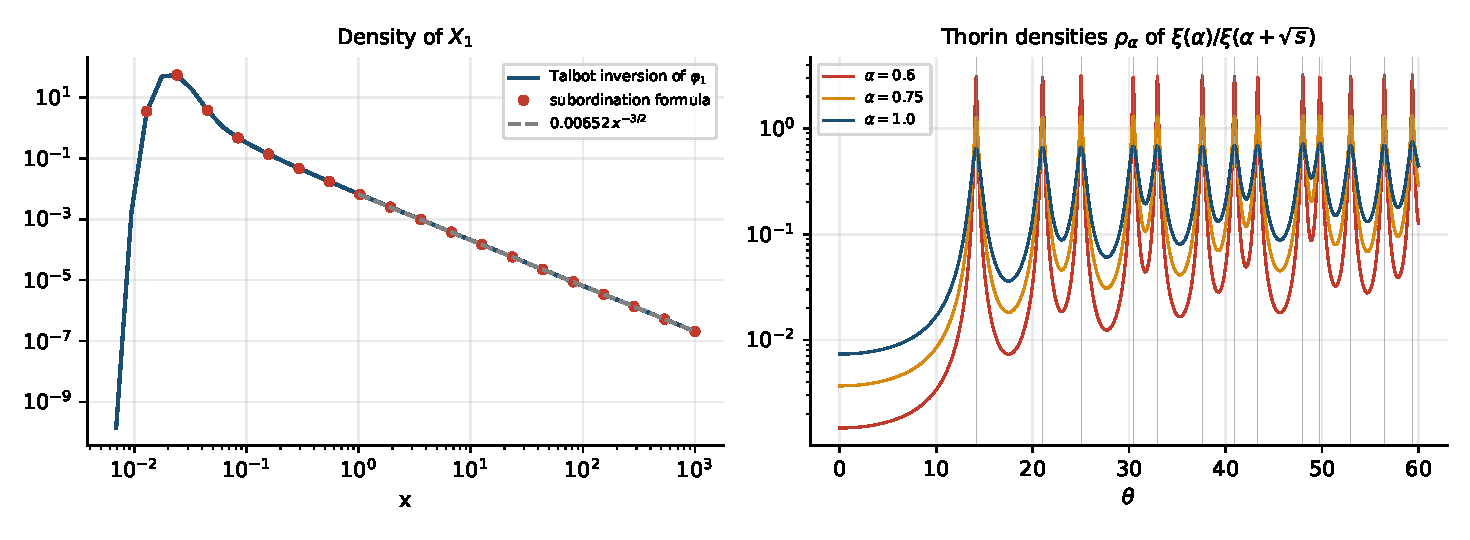
\includegraphics[width=\textwidth]{fig/bp1_density2.pdf}
\caption{Left: the density of $T_1$ by Talbot inversion of $\varphi_1$ and by the subordination formula \eqref{bp:eq:density}, with the tail $0.00652\,x^{-3/2}$. Right: the densities $v_\alpha/\pi$ at the basepoints $\alpha=0.6$, $0.75$ and $1$, with the ordinates of the zeros; they sharpen onto the zeros as $\alpha$ decreases, and for $\alpha<1$ they are Thorin densities of $T_\alpha$ only if no zero lies to the right of the line $\re s=\alpha$. The plots write $X_1$ for $T_1$, $\rho_\alpha$ for $v_\alpha/\pi$ and $s$ for $u$. Drawn by \texttt{figs2.py}.}
\label{bp:fig:density2}
\end{figure}

\label{bp:sec:planar}The Cauchy kernels of Proposition~\ref{bp:prop:thorin} and the stable one half subordinator of Theorem~\ref{bp:thm:sub} are both laws of planar Brownian motion at the moment it first reaches a line. Let $B=(B^1,B^2)$ be a planar Brownian motion started at a zero $\rho=\beta+i\gamma$, identified with the point $(\beta,\gamma)$, and let $H$ be the first time $B^1$ reaches the line $\re s=1$, a distance $1-\beta$ away, that is, the first passage time $H_{1-\beta}$ of the one dimensional Brownian motion $B^1-\beta$. Then $B^2_H$ has the Cauchy law with centre $\gamma$ and width $1-\beta$, which is the harmonic measure of the half plane, and $H$ has Laplace transform $e^{-(1-\beta)\sqrt{2u}}$, the stable one half law. So, exactly,
\[
\rho_{1/2}(\theta)\,d\theta=\sum_\rho P\big(B^2_H\in d\theta\mid B_0=\rho\big).
\]
The times $H$ have the same stable one half law, up to scale, as the stable part of the subordinator $\sigma$ in Theorem~\ref{bp:thm:sub}; the correspondence is of type rather than of scale, since in the theorem the stable part runs per unit of local time $\widetilde T$ rather than per unit of distance.

\subsection{The exact Brownian boundary and Wald's identity}\label{bp:sec:rs1}

The inverse first passage question asks for a boundary $b$ such that the first time $H_b=\inf\{t>0:B_t\ge b(t)\}$ at which a standard Brownian motion started at zero crosses $b$ has the law of $T_1$. A deterministic curved boundary always exists. Anulova proved this for two sided symmetric boundaries \cite{Anulova80}, and Chen, Cheng, Chadam and Saunders for one sided boundaries when the survival function is continuous and positive \cite[Theorem 1]{CCCS11}. By the theorems of Ekstr\"om and Janson \cite[Theorems 2.3, 8.2 and 9.2]{EkstromJanson16}, every law on $(0,\infty)$ is the law of $H_b$ for a lower semicontinuous boundary $b$, which is continuous on every interval where the density of the law is bounded below by a positive constant; when that holds on every compact subinterval of $(0,\infty)$, $b$ is the unique continuous solution of the Volterra equation \eqref{eq:ch19:volterra} with $\liminf_{t\downarrow0}b(t)\ge0$. The density \eqref{bp:eq:density} of $T_1$ is continuous and positive on $(0,\infty)$, so the boundary of $T_1$ is continuous there, and it can be computed from the law of $T_1$ alone through \eqref{eq:ch19:volterra}, with $f$ the density of $T_1$, used in the complementary form of Section~\ref{sec:ch19:zones}, with $P(T_1>t)$ in place of $P(T>t)$, once the survival probability falls below one half; \texttt{rs1.py} solves it. We computed the distribution function of $T_1$ by Talbot inversion of $\varphi_1(u)/u$ for $t<0.03$, where $T_1$ is super flat, and by the subordination representation of Theorem~\ref{bp:thm:sub} beyond, in the form
\[
P(T_1>t)=\E\Big[\mathbf 1\{\widetilde T\ge t\}+\mathbf 1\{\widetilde T<t\}\Big(2\mathcal N\Big(\frac{\widetilde T}{\sqrt{2(t-\widetilde T)}}\Big)-1\Big)\Big],
\]
with $\mathcal N$ the standard normal distribution function, as in Section~\ref{sec:ch19:zones}. This form is smooth and gives the survival function to relative accuracy even at $t=100$, where $\sqrt t\,P(T_1>t)=0.013037$ against the limit $0.013030$. As at the centre, the boundary is computed over the three zones of Section~\ref{sec:ch19:zones}.

In the small time zone the law of $T_1$ near the origin is that of the tilted centre clock, and the boundary starts from the reflection level $0.505$ at $t=0.009$. In the bulk, from $t=0.011$ to $t=0.05$, the boundary falls steeply, to $0.363$ at $t=0.012$ and $0.111$ at $t=0.02$. Here the tangent approximation, taken in its density form, equates the first passage density of the tangent line with the density of $T_1$, where the boundary of Roberts and Shortland \cite{RS95} in Section~\ref{sec:ch19:tangent} equates hazards. Its solution, the boundary $b$ with $(b-tb')(2\pi t^3)^{-1/2}e^{-b^2/2t}=f(t)$ computed by \texttt{rs1c.py}, agrees with the exact boundary to $10^{-4}$ at $t=0.012$ and to $1.5\times10^{-3}$ at $t=0.02$.

The right tail is where the basepoint one differs completely from the centre. At the centre the survival function is exponential and the boundary is asymptotically linear with slope $-\sqrt2\gamma_1$ (Section~\ref{sec:ch19:zones}). At the basepoint one the survival function is the stable one half tail $0.01303\,t^{-1/2}$, and a Brownian motion survives that long only below a boundary that stops moving. The exact boundary flattens at the level $b_\infty=-0.19277$: it stays within $10^{-3}$ of this level from $t=0.056$ on and within $10^{-4}$ from $t=1.2$ on, up to the end of the computation at $t=100$; that $b_\infty=\lim_{t\to\infty}b(t)$ is observed, not proved. The tangent approximation fails here: it overshoots downward, to $-0.332$ at $t=0.05$ against the exact $-0.188$, and has no solution beyond $t=0.091$. It treats the crossing density at time $t$ as if the path had just started, so a flat boundary at level $a$ would have to produce the density $a\,(2\pi)^{-1/2}t^{-3/2}$, forcing $a=\sqrt{2\pi}\times0.00652=0.0163>0$; but by the time the tail is reached the tangent boundary is already negative, and a negative linear boundary can only produce an exponential tail.

The positive number $0.0163$ does appear in the exact picture, in a different role. Optional stopping for the martingale $B_{t\wedge H_b}$ gives $\E[b(H_b)\mathbf 1\{H_b\le t\}]=-\E[B_t\mathbf 1\{H_b>t\}]$, and once the boundary is flat, a survivor at depth $y$ below it survives a further time $r$ with probability about $y\sqrt{2/(\pi r)}$. The next lemma makes the matching of these two facts exact. For a continuous monotone boundary that is positive at $0$ the limit is Theorem~2 of Novikov \cite{Novikov96}; the lemma assumes boundedness in place of monotonicity.

\begin{lemma}\label{bp:lem:wald}
Let $b$ be continuous on $(0,\infty)$ and bounded on $[1,\infty)$, and let $H_b=\inf\{t>0:B_t\ge b(t)\}$ be positive almost surely. Then $b(H_b)=B_{H_b}$ is integrable and $\sqrt t\,P(H_b>t)\to\sqrt{2/\pi}\,\E\,b(H_b)$ as $t\to\infty$.
\end{lemma}

\begin{proof}
Since $b$ is bounded above on $[1,\infty)$ and $\limsup_tB_t=\infty$, $H_b$ is finite, and $B_{H_b}=b(H_b)$ by continuity. Choose $u_0>0$ with $P(H_b>u_0)>0$; on that event $b>B$ on $(0,u_0]$, so $b$, which is also continuous on $[u_0,1]$ and bounded on $[1,\infty)$, is bounded below on $(0,\infty)$, say by $-K$. Optional stopping gives $A(s)=\E[b(H_b)\mathbf 1\{H_b\le s\}]=-\E[B_s\mathbf 1\{H_b>s\}]$. Fix $s\ge1$, let $c_1$ and $c_2$ be the infimum and the supremum of $b$ on $[s,\infty)$, and let $g(y,\tau)=(2\mathcal N(y/\sqrt\tau)-1)^+$, the probability that a Brownian motion started at zero stays below the level $y$ up to time $\tau$. By the Markov property at time $s$, on $\{H_b>s\}$ the conditional probability of $\{H_b>t\}$ given the path up to time $s$ lies between $g(c_1-B_s,t-s)$ and $g(c_2-B_s,t-s)$, and $c_2-B_s>0$ there. Since $\sqrt t\,g(y,t-s)\to\sqrt{2/\pi}\,y^+$ as $t\to\infty$, and $\sqrt t\,g(y,t-s)\le2y^+$ for $t\ge2s$, dominated convergence and $y^+\ge y$ give
\[
\begin{aligned}
\liminf_{t\to\infty}\sqrt t\,P(H_b>t)&\ge\sqrt{\tfrac2\pi}\big(c_1P(H_b>s)+A(s)\big),\\
\limsup_{t\to\infty}\sqrt t\,P(H_b>t)&\le\sqrt{\tfrac2\pi}\big(c_2P(H_b>s)+A(s)\big).
\end{aligned}
\]
The upper bound at $s=1$ and the lower bound at every $s$ bound $A(s)$ uniformly, so, since $b(H_b)\ge-K$, monotone convergence makes $b(H_b)$ integrable with $A(s)\to\E\,b(H_b)$. As $s\to\infty$, $c_1$ and $c_2$ stay bounded and $P(H_b>s)\to0$, so both bounds tend to $\sqrt{2/\pi}\,\E\,b(H_b)$.
\end{proof}

The exact boundary of $T_1$ is continuous; its boundedness on $[1,\infty)$, which the lemma needs, is observed, not proved. Granting it, the lemma and the tail \eqref{bp:eq:tail} give
\[
\E\,b(T_1)=\lim_{t\to\infty}\E\big[(b_\infty-B_t)\mathbf 1\{H_b>t\}\big]=\sqrt{\frac\pi2}\times\frac{\sum_\rho\rho^{-1}}{\sqrt\pi}=\frac{1}{\sqrt2}\sum_\rho\frac1\rho=0.0163311 ,
\]
the first equality by optional stopping, since $P(H_b>t)\to0$. So, if the boundary is bounded on $[1,\infty)$, Wald's identity $\E B_{H_b}=0$, which holds for every crossing time of finite mean, fails here, and the defect is exactly $\sum_\rho\rho^{-1}/\sqrt2$. Numerically, integrating the computed boundary against the law of $T_1$ gives $\E\,b(T_1)=0.0163370$. The defect is also the level of the stable summand of $T_1$: since $\E e^{-uH_a}=e^{-a\sqrt{2u}}$, the variable $S$ of Proposition~\ref{bp:prop:v1min} has the law of the first passage time $H_{b_1/\sqrt2}$ (Section~\ref{ri:sec:kill}).

We simulated $1.5\times10^5$ Brownian paths against the exact boundary on $[0,1]$, with a Brownian bridge crossing correction, using \texttt{rs1d.py}. The Kolmogorov distance between the simulated and the exact survival functions is $0.0019$, at the level of the Monte Carlo noise. Figure~\ref{bp:fig:rs1}, drawn by \texttt{figs5.py}, shows the boundary in its three zones and the survival check.

\begin{figure}[htbp]
\centering
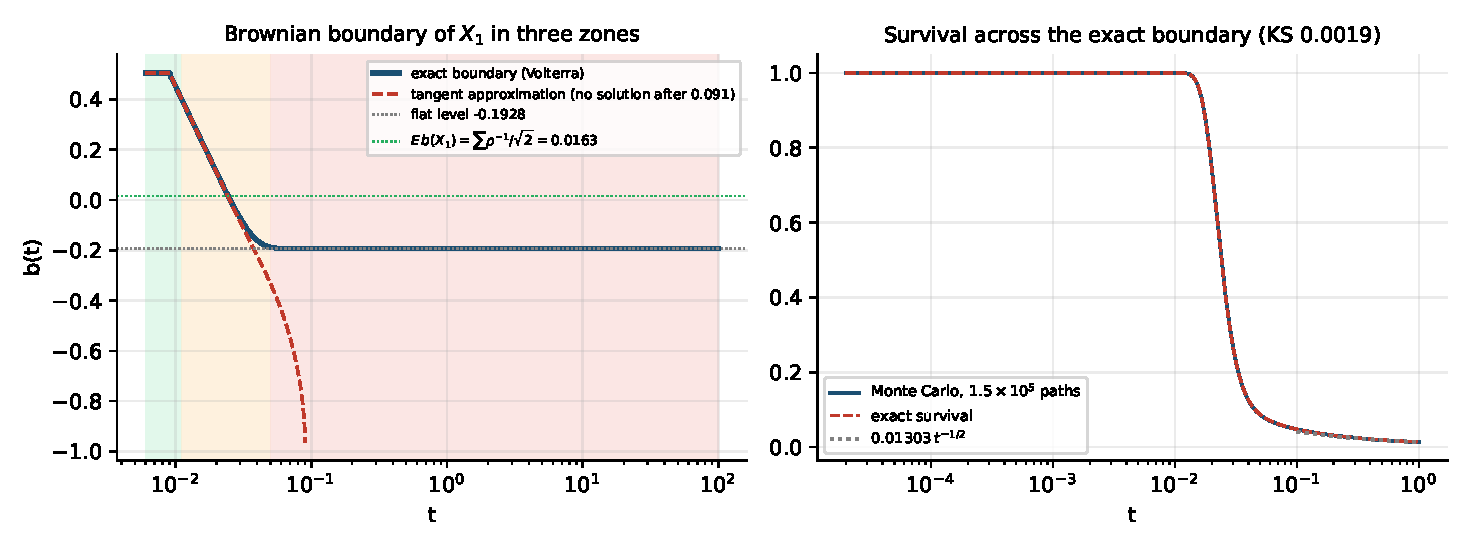
\includegraphics[width=\textwidth]{fig/bp1_rs1.pdf}
\caption{Left: the exact Brownian boundary of $T_1$, written $X_1$ in the plot, from the Volterra equation over the three zones of Section~\ref{sec:ch19:zones} (shaded: small time, bulk, right tail), the tangent approximation, which has no solution beyond $t=0.091$, the flat level $-0.19277$, and the value $\E\,b(T_1)=\sum_\rho\rho^{-1}/\sqrt2=0.0163$. Right: survival of $1.5\times10^5$ simulated Brownian paths across the exact boundary against the exact survival function of $T_1$ and the tail $0.01303\,t^{-1/2}$; the Kolmogorov distance is $0.0019$.}
\label{bp:fig:rs1}
\end{figure}

\subsection{Every basepoint above the centre}\label{bp:sec:alpha}

Nothing in Theorem~\ref{bp:thm:sub} is special to the basepoint one. Since $(\alpha-\frac12+\sqrt u)^2=(\alpha-\frac12)^2+u+2(\alpha-\frac12)\sqrt u$, the same computation applies at every basepoint to the right of the centre.

\begin{theorem}\label{bp:thm:alpha}
For every $\alpha>\frac12$, with no hypothesis on the zeros (the existence of the centre clock, Theorem~\ref{thm:ch12:idsd}, uses the verification of RH below height $1000$), $\varphi_\alpha(u)=\xi(\alpha)/\xi(\alpha+\sqrt u)$ is the Laplace transform of $T_\alpha\stackrel{d}{=}\sigma^{(\alpha)}_{\widetilde T_\alpha}$, where $\widetilde T_\alpha$ is the centre clock tilted by $e^{-(\alpha-\frac12)^2T}$ and $\sigma^{(\alpha)}$ is an independent subordinator with exponent $u+2(\alpha-\frac12)\sqrt u$, that is $T_\alpha\stackrel{d}{=}\widetilde T_\alpha+H_{\sqrt2(\alpha-\frac12)\widetilde T_\alpha}$. The law has infinite mean and $P(T_\alpha>x)\sim\frac{\xi'}{\xi}(\alpha)\,(\pi x)^{-1/2}$. The variable $T_\alpha$ is a GGC if and only if no zero has $\beta>\alpha$, in particular for every $\alpha\ge1$, and when every zero has $\beta<\alpha$ its Thorin density in the chart $\theta=\sqrt z$ is $\frac1\pi\sum_\rho(\alpha-\beta)/((\alpha-\beta)^2+(\theta-\gamma)^2)$.
\end{theorem}

\begin{proof}
The subordination is the computation of Theorem~\ref{bp:thm:sub} with $\frac14$ replaced by $(\alpha-\frac12)^2$ and $\sqrt u$ by $2(\alpha-\frac12)\sqrt u$, and $H_a$ has exponent $a\sqrt{2u}$ with $a=\sqrt2(\alpha-\frac12)\ell$. The tail follows as in Section~\ref{bp:sec:thorin} from $\varphi_\alpha(u)=1-\frac{\xi'}{\xi}(\alpha)\sqrt u+O(u)$. The Thorin density and the GGC criterion are the threshold theorem, Theorem~\ref{thm:poisson}: when every zero has $\beta<\alpha$ each Cauchy term is positive, and a zero with $\beta>\alpha$ puts a pole of $\varphi_\alpha$ at the point $(\rho-\alpha)^2$ of $\cut$ (its principal root is $\rho-\alpha$, since $\re(\rho-\alpha)>0$), where the Laplace transform of a GGC is holomorphic, whatever the sign of the density near its ordinate (Remark~\ref{rem:ch2:oneline}). In the boundary case, when some zero has $\beta=\alpha$ and none has $\beta>\alpha$, every zero has $\beta<\alpha'$ for $\alpha'>\alpha$, so $T_{\alpha'}$ is a GGC; as $\alpha'\downarrow\alpha$, $\varphi_{\alpha'}\to\varphi_\alpha$ pointwise on $[0,\infty)$, so $T_{\alpha'}\to T_\alpha$ in law, and $T_\alpha$ is a GGC by the closure theorem of Section~\ref{sec:weak:limits}. There the Cauchy kernel of a zero $\alpha+i\gamma$, $\gamma>0$, of multiplicity $m$ becomes an atom: with its conjugate it contributes the factor $(1+u/\gamma^2)^{-m}$ to $\varphi_\alpha$, a Thorin atom of mass $m$ at $z=\gamma^2$.
\end{proof}

\begin{corollary}\label{bp:cor:levyalpha}
Let $\alpha>\frac12$ and $a=\alpha-\frac12$. Then $T_\alpha$ is infinitely divisible, with no drift and L\'evy measure $W_\alpha(x)\,dx/x$, where
\begin{align*}
W_\alpha(x)&=\frac{ax}{\sqrt\pi}\int_0^x(x-s)^{-3/2}e^{-a^2xs/(x-s)}\,W(s)\,ds\\
&=\E\Big[(1+4xV)^{-1/2}\,W\Big(\frac x{1+4xV}\Big)\Big],
\end{align*}
with $V=a^2/(2Z^2)$ and $Z$ standard normal. Hence $W_\alpha>0$ and $W_\alpha'<0$ on $(0,\infty)$, so that $T_\alpha$ is self decomposable; and on every interval $(0,T]$ on which $W$ is completely monotone, so is $W_\alpha$.
\end{corollary}

\begin{proof}
By Theorem~\ref{bp:thm:alpha}, $T_\alpha$ is the subordinator $\sigma^{(\alpha)}_s=s+H_{\sqrt2as}$ evaluated at the independent time $\widetilde T_\alpha$, which is infinitely divisible with no drift and L\'evy measure $e^{-a^2s}W(s)\,ds/s$, and $H_{\sqrt2as}$ has the density $(as/\sqrt\pi)y^{-3/2}e^{-a^2s^2/y}$. By Bochner's subordination \cite[Theorem 30.1]{Sato99}, $T_\alpha$ is infinitely divisible with no drift and L\'evy measure $\int_0^\infty P(\sigma^{(\alpha)}_s\in dx)\,e^{-a^2s}W(s)\,ds/s$, which, since $a^2s^2/(x-s)+a^2s=a^2xs/(x-s)$, is $W_\alpha(x)\,dx/x$ with the first form of $W_\alpha$. The substitution $s=x/(1+4xv)$ turns the integral into an average against the density $\frac a{2\sqrt\pi}v^{-3/2}e^{-a^2/4v}$ of $V$, which is the second form. There the derivative in $x$ of $(1+4xv)^{-1/2}W(x/(1+4xv))$ is $-2v(1+4xv)^{-3/2}W+(1+4xv)^{-5/2}W'$, negative because $W>0$ and $W'<0$ (Theorem~\ref{thm:ch12:idsd}), and differentiation under the average is legitimate, because $W^{(n)}(s)=O(s^{-n-1/2}\log(1/s))$ as $s\to0$ makes every derivative in $x$ of the integrand $O(\log(1+V))$ on compact subsets of $(0,\infty)$, and $\E\log(1+V)<\infty$. Finally, $x\mapsto x/(1+4xv)$ has a completely monotone derivative and maps $(0,T]$ into itself, and $(1+4xv)^{-1/2}$ is completely monotone, so Fa\`a di Bruno's formula and Leibniz's rule carry complete monotonicity of $W$ on $(0,T]$ to every term of the average.
\end{proof}

With Theorem~\ref{thm:ch12:cmint}, $W_\alpha$ is therefore completely monotone on $(0,1.29]$ for every $\alpha>\frac12$. When no zero has real part above $\alpha$, in particular for every $\alpha\ge1$, $T_\alpha$ is a GGC and $W_\alpha$ is the Laplace transform $k_\alpha$ of its Thorin measure (Section~\ref{pm:sec:wg}); when some zero has real part above $\alpha$, $T_\alpha$ is not a GGC, so $W_\alpha$ is not completely monotone on $(0,\infty)$, although it is on $(0,1.29]$.

Table~\ref{bp:tab:alpha}, computed by \texttt{improve.py}, and the right panel of Figure~\ref{bp:fig:density2} give the constants and the densities for three basepoints. As $\alpha\downarrow\frac12$ the tail constant $\frac{\xi'}{\xi}(\alpha)/\sqrt\pi$ tends to zero, because $\xi'(\frac12)=0$, and the law acquires the finite mean $\sum_ka_k^{-1}$ of the centre clock; at the same time the subordinator tends to pure drift and the Cauchy widths to $\frac12-\beta$, which is where RH is decided.

\begin{table}[htbp]
\centering\small
\begin{tabular}{cccc}
\toprule
$\alpha$ & $\frac{\xi'}{\xi}(\alpha)$ & tail constant $\frac{\xi'}{\xi}(\alpha)/\sqrt\pi$ & $\min_{[0,60]}\rho_{\alpha-1/2}$\\
\midrule
0.6 & 0.00462092 & 0.002607 & 0.00147\\
0.75 & 0.01155134 & 0.006517 & 0.00368\\
1 & 0.02309571 & 0.013030 & 0.00735\\
\bottomrule
\end{tabular}
\caption{Basepoints above the centre: the drift $\frac{\xi'}{\xi}(\alpha)$, the tail constant of $T_\alpha$, and the minimum on $[0,60]$, attained at the origin, of the density $\rho_{\alpha-1/2}=v_\alpha/\pi$, the Thorin density of $T_\alpha$ when every zero lies to the left of the line $\re s=\alpha$. At $\alpha=1$ the minimum at the origin holds at every height (Proposition~\ref{bp:prop:v1min}), as it does at every $\alpha\ge1$ (Proposition~\ref{bp:prop:valpha}); for $\frac12<\alpha<1$ the minimum at the origin holds on the verified window $|\theta|\le3\times10^{12}-1.21$ (Theorem~\ref{thm:dbeta:minall}(ii)), and at every height for every such $\alpha$ it is equivalent to RH (part (vi) of that theorem).}
\label{bp:tab:alpha}
\end{table}

\subsection{Boundaries across the basepoints}\label{bp:sec:across}

We solved the Volterra equation \eqref{eq:ch19:volterra} \cite{Peskir02} at $\alpha=0.6$ and $0.75$, with the law of $T_\alpha$ from Theorem~\ref{bp:thm:alpha}. As at the basepoint one, the distribution function comes from Talbot inversion of $\varphi_\alpha(u)/u$ for $t<0.03$ and from the subordination identity beyond, here with $3\times10^5$ draws of $\widetilde T_\alpha$, made under RH as a sum of exponential variables over the first $200$ zeros and a gamma variable with the mean and variance of the remaining terms. The bottom left panel of Figure~\ref{pm:fig:paths} in Section~\ref{ch:sato} draws the four boundaries together.

In the small time zone and the bulk the boundaries at the different basepoints are close: they start near the reflection level $0.50$, and at $t=0.02$ they are at $0.072$ for the centre and at $0.080$, $0.092$ and $0.111$ for $\alpha=0.6$, $0.75$ and $1$. They differ in the right tail. At the centre the survival function is exponential with rate $\gamma_1^2$, and the boundary is asymptotically linear with slope $-\sqrt2\gamma_1=-19.99$ and the logarithmic correction $\frac{3}{2\sqrt2\gamma_1}\log t$; the slope of the computed boundary over $[0.2,0.3]$ is $-19.77$ (Section~\ref{sec:ch19:zones}). Above the centre the exact boundaries flatten: each stays within $0.011$ of its level at $t=100$, the end of the computation, from $t=0.1$ on, and within $10^{-3}$ from $t=1$ on. As $\alpha\downarrow\frac12$ the flat level moves down, towards the linear boundary of the centre.

The Wald type identity of Section~\ref{bp:sec:rs1} extends to every basepoint above the centre. The density of $T_\alpha$ is again continuous and positive on $(0,\infty)$, so its boundary is continuous \cite[Theorem 8.2]{EkstromJanson16}, and as computed it is bounded up to $t=100$. Granting boundedness at infinity, which here too is observed, not proved, Lemma~\ref{bp:lem:wald} and the stable tail $P(T_\alpha>t)\sim b_\alpha(\pi t)^{-1/2}$ of Theorem~\ref{bp:thm:alpha} give $\E\,b(T_\alpha)=b_\alpha/\sqrt2$, so Wald's identity $\E B_{H_b}=0$ fails by exactly $b_\alpha/\sqrt2$. Table~\ref{bp:tab:across} compares the identity and the tail constant with the computed values; all six pairs agree to within $6\times10^{-4}$ in relative terms. The reason given in Section~\ref{bp:sec:rs1} for the failure of the tangent approximation in the right tail holds at every basepoint above the centre.

\begin{table}[htbp]
\centering\small
\begin{tabular}{cccccc}
\toprule
$\alpha$ & flat level & $\E\,b(T_\alpha)$ & $b_\alpha/\sqrt2$ & $\sqrt{100}\,P(T_\alpha>100)$ & $b_\alpha/\sqrt\pi$\\
\midrule
0.6 & $-0.33384$ & 0.0032687 & 0.0032675 & 0.0026083 & 0.0026071\\
0.75 & $-0.25537$ & 0.0081710 & 0.0081680 & 0.0065203 & 0.0065171\\
1 & $-0.19277$ & 0.016337 & 0.016331 & 0.013037 & 0.013030\\
\bottomrule
\end{tabular}
\caption{Exact Brownian boundaries above the centre: the flat level, the mean boundary value $\E\,b(T_\alpha)$ at the crossing, obtained by integrating the computed boundary against the law of $T_\alpha$, against the Wald type identity, and the computed $\sqrt{100}\,P(T_\alpha>100)$ against the tail constant of Theorem~\ref{bp:thm:alpha}. Computed by \texttt{bnd\_alpha.py} for $\alpha=0.6$ and $0.75$ and by \texttt{rs1.py} for $\alpha=1$.}
\label{bp:tab:across}
\end{table}
